\subsection{Итеративный метод}
Если не удается вычислить оптический поток за одну итерацию, то можно применять итеративный метод.  Суть метода заключается в следующем :  имеются одномерные функции $f_1(x)$ на первом кадре и $f_2(x)$ —  на втором. Необходимо найти вектор смещения $d$. Функция $f_1(x)$ преобразуется с помощью замены значения в точке x на смещенное значение.

Недостатки данного подхода. В случае нахождения смещенного значения меньше целого пикселя, невозможно сместится на данное значение. Можно проинтерполировать значения на втором изображении с учетом найденного смещения.
 
\subsection{Иерархический метод}
Пирамидальный (иерархический) алгоритм Лукаса - Канаде в значительной степени использует классический метод. В методе используется пирамида изображений т.е. последовательность изображений, в которой каждое последующее получается из предыдущего уменьшением его размеров в два раза.

Каждое изображение последовательности, за исключением первого, получается как свертка предыдущего изображения со следующим фильтром:
(рис. \ref{pic:pyramid}).
Пирамидальный алгоритм Лукаса - Канаде для поиска потока в точке $(x_0,y_0)$. 
\begin{enumerate}
\item По каждому из двух данных изображениям строится пирамида изображений
\item Для $i$ – го изображения пирамиды по первому и второму изображениям применяется классический KLT метод, с вектором начального приближения $2 \cdot d_{i+1}$, где $d_{i+1}$ – вектор потока, полученный на предыдущем уровне пирамиды.
\end{enumerate} 
Для самого первого уровня этот вектор принимается равным (0,0).


\begin{figure}[ht]
\center{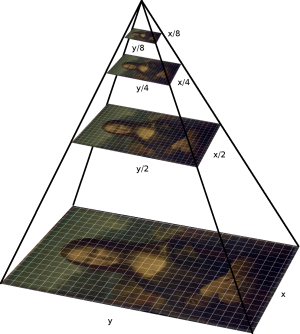
\includegraphics[width=0.6\linewidth]{pyramid}}
\caption{Пример пирамиды Гаусса}
\label{pic:pyramid}
\end{figure}